\section{Durchführung}
\label{sec:Durchfuehrung}
\subsection{Versuchsaufbau}
\begin{figure}[ht]
    \centering
    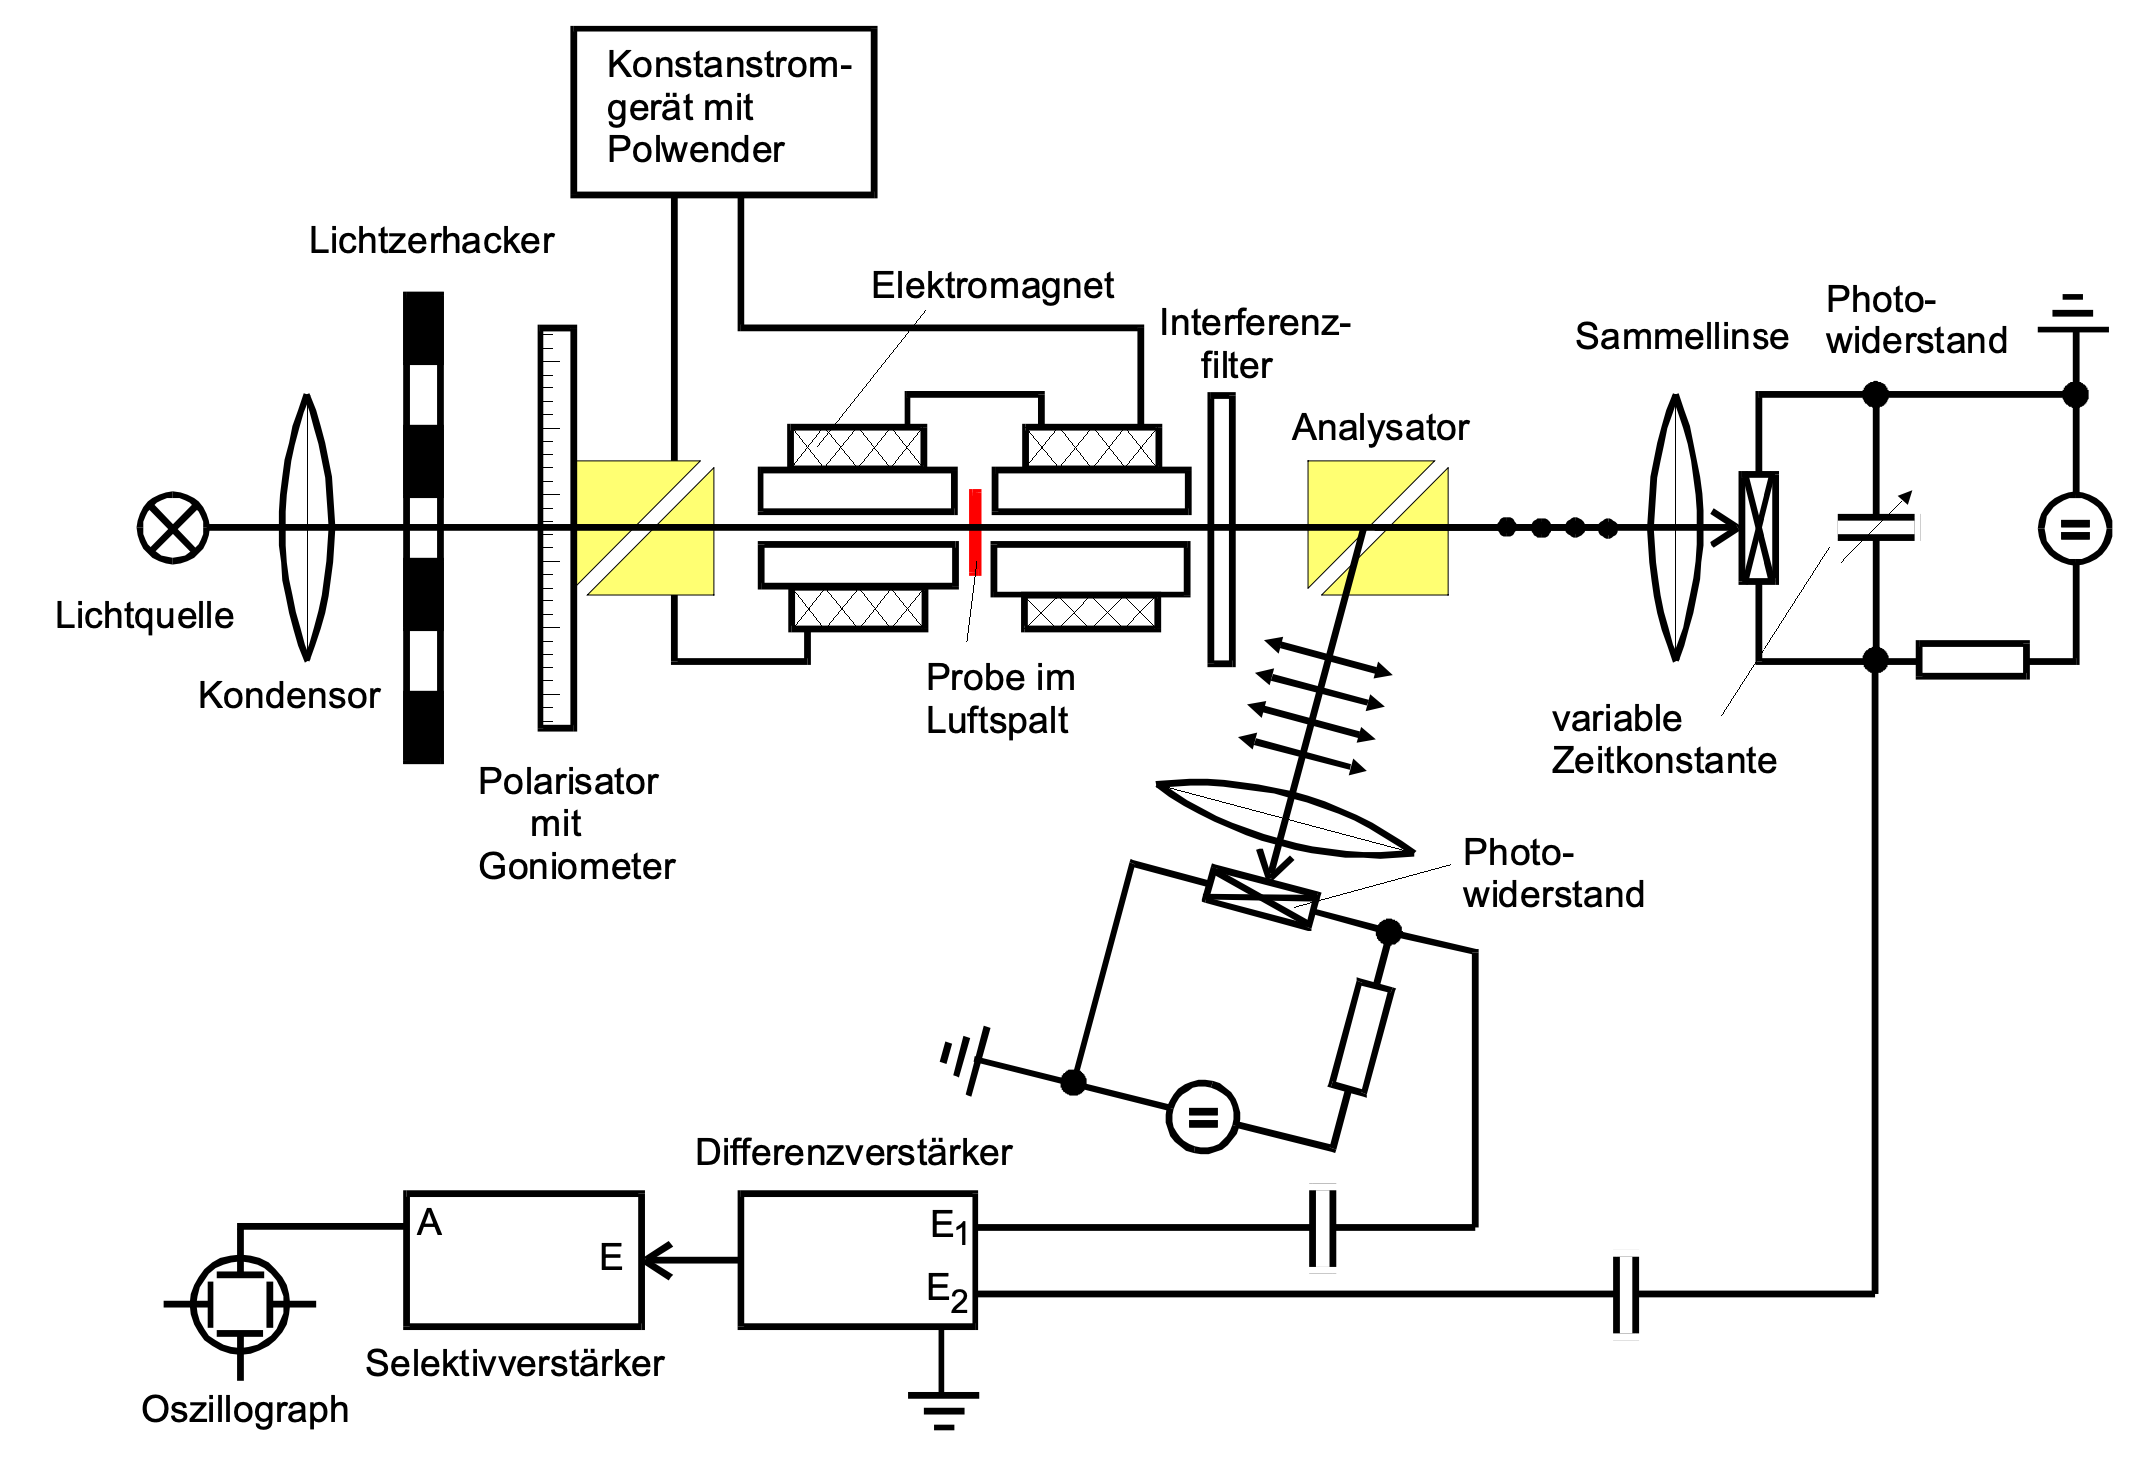
\includegraphics[width = 0.75 \textwidth]{./bilder/Schematische_Darstellung_der_Messapparatur.png}
    \caption{Versuchsaufbau}
    \label{fig:aufbau}
\end{figure}
Der Weg des Lichtes durch den Aufbau startet in Abbildung \ref{fig:aufbau} bei der Lichtquelle, in diesem Fall eine Halogenlampe im Infraroten Bereich.
Mithilfe eines Kondensators wird der Lichtstrahl parallel ausgerichtet um nun als parallele Strahlen den Aufbau durchlaufen.
Dieser Strahl durchläuft anschließend einen Zerhacker, der den Lichtstrahl in Pulse mit einer eingestellten Frequenz aufspaltet.
Das nun parallele Licht trifft auf das erste Glan-Thompson-Prisma mit einem Goniometer zu Winkeleinstellung und wird dabei in zwei Strahlen aufgespaltet von dem nur ein linear Polarisierter verwendet wird.
Dieser linear polarisierte Strahl durchläuft die Probe zwischen den Elektromagneten zur Messung des Faraday-Effekt.
Nach dem Durchlaufen der Elektromagneten fällt der Strahl auf einen Interferenzfilter der das Licht monochromatisiert.
Während des Versuchs wird mit verschiedenen Interferenzfiltern der Faraday Effekt für verschiedene Wellenlängen des Lichts untersucht.
Mithilfe eines weiteren Glan-Thompson-Prismas wird der monochromatische Strahl nun in zwei zueinander senkrecht Polarisierte Strahlen zerteilt und weiter analysiert.
Die beiden Strahlen treffen auf jeweils eine Sammellinse die die Strahlen auf einen jeweiligen Photowiederstand fokussiert.
Die beiden Signale der Photowiederstände werden mit einer Schaltung eines Differenzverstärkers verbunden, der eine Spannung proportional zur Differenz der Eingangsspannungen ausgibt.
Das Signal passiert anschließend einen Frequenzverstärker der auf die Zerhackerfrequenz des Aufbaus eingestellt ist.
\subsection{Justierung der Apparatur}
Zunächst wird der Aufbau komplett justiert damit die zwei Strahlen nach dem zweiten Glan-Thompson Prisma auf die beiden Photowiederstände treffen.
Diese Justage findet visuell statt indem der Strahlengang beobachtet wird und genau eingestellt wird.
Zur Justierung wird daher zunächst die Probe und der Interferenzfilter entfernt um den richtigen Strahlengang durch die Magnete und die Probe zu gewährleisten und sichtbares Licht zur verfügung zu haben.
Um das Rauschen des Hintergrundes für das Signal zu minimieren wird anschließend die Frequenz für den Frequenzverstärker auf die Zerhackerfrequenz eingestellt und eingestellt um das Ausgangssignal zu maximieren.
\subsection{Magnetfeldmessung}
Mithilfe einer Hall Sonde wird das Magnetfeld innerhalb der Spulen gemessen.
Die Messung ist zwingend notwendig, da der Faraday Effekt proportional zu magnetischen Flussdichte am Ort der Probe ist.
Mit einer Messapparatur mit millimetereinstellung und Hall Sonde wird die Flussdichte zentriert um den ort der Probe vermessen.
\subsection{Winkelmessungen}
Zur Messung der Faraday-Rotation wird mit der maximalen Feldstärke $B_{max}$ gemessen.
Anschließend wird ein Winkel $\theta_1$ eingestellt für den das Ausgangssignal verschwindet.
Nach dem umpolen des Magnetfeldes,wird das erste Prisma nun bis zu einem Winkel $\theta_2$ gedreht an dem das Signal erneut verschwindet.
Der gesamte Rotationswinkel ergibt sich damit zu 
\begin{equation*}
    \theta = \frac{\theta_1 - \theta_2}{2}
\end{equation*}
Diese Messung wird für die verschiedenen Proben, Probendicken und Interferenzfilter wiederholt und dokumentiert.
